\documentclass[a4paper,fleqn]{cas-dc}
\usepackage[numbers,sort&compress]{natbib}
\usepackage{tabularx,longtable,adjustbox,placeins}
\usepackage{lmodern,microtype}
\hypersetup{hidelinks}
\setlength{\emergencystretch}{1em}
\graphicspath{{figures/}}
\newcommand{\ind}{\mathbf{1}}
\begin{document}
\let\WriteBookmarks\relax
\shorttitle{Deadline-Limited Communication in MARL}
\shortauthors{Kung and Ha}
\title[mode=title]{Evaluating Deadline-Limited Communication in Multi-Agent Reinforcement Learning: Delivery, Computation, and Control}
\author{Yeong-woo Kung}
\author{Young-guk Ha}
% Affiliations, corresponding author and declarations await author input.
\begin{abstract}
Reducing message traffic while preserving cooperative return can justify a smaller communication budget. It gives little guidance on which messages to suppress or whether the receiver needs to change. We study these decisions in multi-agent reinforcement learning by matching policies and episodes and tracing each offered message to the action deadline. In a published image-based addition game, all three reconstructed speaker--listener policies learned useful communication. Under a modeled 750-microsecond reception deadline, omitting only packets known to arrive late halves offered traffic and preserves the listener's action distribution on every example. At the same mean byte budget, random admission reduces expected correct-sum accuracy from 29.37\% to 18.78\% (paired difference 10.59 percentage points, 95\% interval [7.25, 13.92]). In a separate hidden-source broadcast task, the received messages contain information the acting policy uses only partly. Supervised adaptation of the follower head at fixed packet readiness improves return by 1.29 points per 20-step episode [0.66, 1.91] across ten seeds. Five-agent Hallway supplies a boundary case: round-robin access saves 80\% of offered bytes with identical control histories when one packet fits in aligned order. When two packets fit, equal packet counts conceal different sender histories in every pair. Together these results identify which observations support changing admission, sender selection or the receiver in the conditions studied.
\end{abstract}
\begin{keywords}
Multi-agent reinforcement learning \sep Communication scheduling \sep Deadline constraints \sep Message selection \sep Controlled evaluation
\end{keywords}
\renewcommand{\printorcid}{}
\maketitle
\section{Introduction}
Communication-efficient multi-agent reinforcement learning seeks to retain cooperative performance while reducing message exchange. VBC pursues this objective through variance-based control, while TMC uses temporal smoothing to reduce communication and improve robustness to transmission loss~\citep{zhang2019efficient,zhang2020succinct}. SchedNet learns which agents access a shared medium~\citep{kim2019schedule}. Their shared goal motivates a more specific evaluation question: when fewer transmissions accompany maintained return, what establishes the contribution of message selection?

Consider five agents that each offer one packet to a channel that can deliver only the first before they act. A scheduler that offers just that packet cuts traffic by 80\%. If the receiver obtains the same payload at the same time on every step, the change cannot improve its decisions. Now let two packets fit. Two schedulers may deliver the same number of packets and still update different entries in the receiver's cache. The difference can persist after the scheduler next makes the same choice. In our five-agent Hallway experiment both situations occur with the same pair of access rules.

This raises two questions for an evaluator. When throughput falls and return is maintained, what evidence establishes that a particular admission or sender choice preserved useful information? When messages arrive on time, what evidence justifies changing the receiver? Our primary quantity is the expected difference in return per episode under a specified change. We track offers, timely deliveries, sender identities and timestamps on matched policies and resets. Where the simulator permits, we also branch at the same decision point to measure the effect of a feasible sender choice after an identical history.

Two learned communication tasks illustrate how the diagnosis changes a design decision. In the MNIST-sum game of \citet{eccles2019biases}, a message intervention establishes that the listener uses the channel. A further comparison at equal offered cost measures how much of this benefit survives a modeled deadline when the scheduler chooses which packets to admit. In hidden-source broadcast, a decoder fitted to the messages arriving under ordinary access predicts the current source bit more accurately than the acting receiver. We test that explanation by changing only the follower head and measuring return on fresh episodes. Hallway then lets us examine when packet counts, cache initialization and the computation of sender priorities change the interpretation of a traffic--return comparison.

\section{Related Work}
\paragraph{From communication reduction to sender selection}
Learned channels, aggregation and targeted messages support cooperative policies~\citep{foerster2016learning,sukhbaatar2016learning,das2019tarmac}, while IC3Net learns when to communicate~\citep{singh2019learning}. VBC studies communication efficiency through variance-based control~\citep{zhang2019efficient}. TMC reports reduced exchange with maintained performance and robustness to transmission loss~\citep{zhang2020succinct}; ETCNet explicitly imposes a bandwidth constraint~\citep{hu2023event}. These are communication-efficiency objectives. Our Full--RR identity comparison asks the narrower attribution question: can the same traffic reduction arise without changing any received information?

SchedNet learns shared-medium access and compares against round-robin scheduling~\citep{kim2019schedule}; IMAC addresses efficient communication through an information bottleneck~\citep{wang2020imac}. Graph attention, teammate modeling and importance-aware exchange add richer selection mechanisms~\citep{liu2020game,yuan2022incentive,huang2024qmnet}, alongside model-based sparsity and asynchronous scheduling~\citep{han2023model,han2025sparse,srinivasan2025asynchronous}. These approaches motivate our fixed-packet-count subset and common-prefix comparisons: an episodic scheduler difference can combine sender choice with a changed information history. We evaluate that ambiguity on a shared GRU/QMIX backbone~\citep{rashid2018qmix}. \citet{zhu2024survey} review the broader design space.

\paragraph{From fresh delivery to useful control}
DACOM learns how long an agent should wait for messages~\citep{yuan2023dacom}. We examine the complementary cost of preparing those messages and selecting their senders before reception begins. In distributed inference, \citet{jung2023splitting} jointly select computation nodes and data-transfer paths, accounting for transmission, computation and waiting in end-to-end latency. This joint cost perspective motivates our separation of CPU preparation, channel waiting and timely message delivery in MARL evaluation. Age-of-information work measures update freshness~\citep{kaul2012real,liu2022optimizing,gong2022hierarchical,alibotaiken2026freshness}; task-oriented control scheduling connects transmission decisions to control objectives~\citep{ayan2022semantics}. Freshness and information use therefore require separate observations. \citet{lowe2019pitfalls} distinguish signaling from listening and show why coarse communication metrics can mislead. For our comparison, an intervention on the message received measures how the frozen listener responds. It does not specify which attempted messages the deployment rule could deliver. Recording the realized delivery history and comparing admission rules at the same offered cost supply that missing comparison. In the MNIST-sum game we evaluate the prior message intervention and the added delivery control on the same pair of policies.
\section{Evaluation Contract and Access Rules}
\subsection{Policy, channel and cost boundary}
In Hallway and broadcast, agents $i\in\{0,\ldots,N-1\}$ share a GRU with local input $[o_i^t;\operatorname{onehot}(a_i^{t-1});e_i]$, where $e_i$ is the agent identifier. A linear head maps hidden state $h_i^t$ to message $m_i^t$. Received messages condition the action head, not the recurrent update. Each message has eight float32 entries: payload $P=32$ B and modeled header 16 B, hence wire size $S=48$ B. Evaluation return is undiscounted $\sum_t r_t$; learning uses discount 0.99.

CPU inference uses one PyTorch thread and \texttt{perf\_counter\_ns}. Measured computation $C_t$ includes encoding, gate selection, serialization, cache operations, transport arithmetic, aggregation, action output and residual bookkeeping; environment stepping and logging are outside this boundary. Tensor-to-byte serialization is charged. If $P_{\mathrm{ready},t}$ is elapsed CPU time at packet readiness, a fixed reserve $R_{\rm post}=0.45$ ms defines $D_{\rm recv}=D_{\max}-R_{\rm post}$. The reserve does not replace actual post-reception computation.

Attempted senders $\mathcal S_t$ are queued by $(i-t)\bmod N$, regardless of priority score. For $K_t=|\mathcal S_t|$, bandwidth $B$ and fixed latency $\ell=0.05$ ms,
\begin{align}
 A_{k,t}&=P_{\mathrm{ready},t}+kS/B+\ell,\nonumber\\ d_{k,t}&=\ind[A_{k,t}\le D_{\rm recv}],\\
 W_t&=\begin{cases}\min\!\left\{\begin{aligned}&K_tS/B+\ell,\\&[D_{\rm recv}-P_{\mathrm{ready},t}]_+\end{aligned}\right\},&K_t>0,\\0,&K_t=0,\end{cases}\\
 T_{\rm step,t}&=C_t+W_t.\label{eq:step}
\end{align}
Accepted broadcasts reach every receiver except the sender. Every attempted packet is charged in full, including cutoff drops; each step flushes the queue. The model has no losses, collisions, retransmissions, acknowledgments or inter-step backlog. Computation and modeled waiting add without overlap: this is hybrid accounting, not measured radio latency. A deadline miss occurs when $T_{\rm step,t}>D_{\max}$; the cutoff cannot eliminate arbitrary CPU jitter.

\subsection{Cache and accounting}
Delivery replaces sender $j$'s cache with $m_j^t$ and its source timestamp with $t$; otherwise both persist. Initially caches are zero and invalid. Validity $v_j^t$ distinguishes never-received entries from fresh zero payloads; receiver age $\tau_j^t$ is time since the valid source timestamp. For receiver $i$,
\begin{equation}
 g_i^t=\frac{\sum_{j\ne i}v_j^t\lambda^{\tau_j^t}c_j^t}{\max(1,\sum_{j\ne i}v_j^t)}.
\end{equation}
The action head uses $[h_i^t;g_i^t;\log(1+\bar\tau_i^t);n_i^t/(N-1)]$, with valid-neighbor count $n_i^t$ and mean valid age $\bar\tau_i^t$. The denominator counts valid senders, not decay weights. Thus delivery changes content, aggregate scaling and metadata together; it is not a pure content intervention.

For measured steps $\mathcal T$ and received count $M_t$, offered load, payload goodput and waste are
\begin{equation}
\begin{aligned} L_{\rm off}&=\frac{S\sum_tK_t}{|\mathcal T|}, &G_{\rm pay}&=\frac{P\sum_tM_t}{|\mathcal T|},\\ \rho_{\rm drop}&=1-\frac{\sum_tM_t}{\sum_tK_t}.\end{aligned}
\end{equation}
Each broadcast is counted once, not per receiver. Waste is undefined when no packets are attempted. Return, load, goodput, cache validity/age, computation and deadline misses measure different outcomes.
\paragraph{Access rules}
Full offers every sender in rotating order. Periodic offers alternating senders. Round-robin (RR) advances through senders in order, subject to link capacity and a byte-credit cap. The priority heuristic (DAC) uses the same cap and ranks senders by their local action-value gap plus a transmitter-age term. The cap charges attempted bytes. A late packet has a cost even when it never reaches the receiver. In matched-history tests both policies use the same cache decay. Supplementary Section~S1 gives the cap, decay and tie-breaking rules.
\section{Experimental Design}
Our primary outcome is the expected difference in undiscounted return per deployed episode. We average paired episodes within each independently trained seed, then weight seeds equally. A second question asks how sensitive a visited state is to substituting a sender for one decision. Longer episodes contribute more states to this latter estimate. We chose the deployment estimand after the original Hallway analysis and before fitting the new broadcast receiver heads. The Supplement reports both weighting schemes and the underlying seed comparisons.

For $n$ trained seeds, $E_s$ matched resets for seed $s$, and intervention $u$ relative to reference $v$, we report the paired episode effect
\begin{equation}
 \widehat{\Delta}_{u,v}=\frac{1}{n}\sum_{s=1}^{n}\frac{1}{E_s}
       \sum_{e=1}^{E_s}\bigl(G_{s,e}^{u}-G_{s,e}^{v}\bigr).
 \label{eq:episode_effect}
\end{equation}
Here $G$ is undiscounted episode reward. The two policies in a closed-loop comparison start at the same reset and subsequently act on their own histories. A changed action can therefore change later observations and messages. We report task reward as scored by the environment and record action-deadline misses separately. No additional fallback action or penalty is imposed on a missed deadline. In the one-step image game we compute $G$ exactly under the stochastic policies for each sampled image pair. In broadcast we observe $G$ by executing all 20 steps.

We use three tasks for distinct questions. In the published MNIST-sum game, a listener must choose the sum of two digits while seeing only its own image and the speaker's message. This supplies an external check on admission and message use. In five-agent broadcast, only the source observes the fresh random bit on each step. Four followers predict it for 20 steps, with reward equal to the fraction correct. A follower without information about the current bit has expected accuracy of one half. We use this task to check whether changing the receiver improves performance at the same access schedule.

In five-agent Hallway, members of each group must reach their destination together within 14 steps. If both groups arrive on the same step, a penalty reduces the combined reward. Each successful group earns 10. A controller with local distances and a public clock earns the full 20 without communication on every one of the 1,024 initial states. The learned ideal-link policies achieve 11.44--12.20 with privileged Oracle demonstrations. This cohort has no prospectively declared absolute learning threshold. Its matched rollouts test which information changes when sender order or cache history changes. We keep the indirect evidence from these policies separate from the learned external and broadcast comparisons.

For Hallway and broadcast we report signed paired effects across seeds. We compare measured CPU readiness with a fixed preparation time of 0.5 ms for admission and delivery, while continuing to record computation. Slow and Medium links provide 20,000 and 100,000 B/s, respectively. Virtual readiness holds reception opportunity fixed. The external task has its own one-packet timing model. Supplementary Sections~S1--S5 give training settings, seed distributions, replay checks and the SMACv2 feasibility record.
\paragraph{Implementation and verification}
OpenAI Codex assisted with experiment implementation, checkpoint evaluation and plotting code. The external admission analysis was checked by independently summing the frozen policies' action and message probabilities on the saved image pairs. For the sequential tasks, the checks compare actions, rewards, deliveries and timestamps in replayed trajectories and verify the pairing of the receiver intervention episodes. The figures summarize logged seed-level outcomes.

\section{Results}
\subsection{Choosing which messages to admit on the external MNIST-sum game}\label{sec:eccles}
In the one-step task of \citet{eccles2019biases}, each agent observes a different MNIST digit image. The speaker chooses one of 20 discrete messages. The listener observes its own image and the message and chooses among 19 possible sums. Both earn one for the correct sum. Conditioning on the listener's digit alone leaves the speaker's digit unknown. The published comparison therefore provides an external case where communication has decision value, and directly addresses positive listening. Each episode has one sender and no cache history. The same-count sender and shared-prefix controls apply to Hallway, not to this game.

We reconstructed the two convolutional policies and independent REINFORCE updates from the paper and its supplement. Both training arms can send a message. The both-bias arm adds losses that encourage the speaker to condition its symbol on its image and the listener to condition its action on that symbol. The no-bias arm omits these auxiliary objectives. Both-bias and no-bias arms use three matched initialization seeds and the same image-pair streams. The two networks have 32- and 64-channel convolutions with kernel 5, pooling and a 1,024-unit hidden layer. The listener concatenates the one-hot symbol after the convolutional encoder. Adam uses learning rate 0.0003 and batches of 32. Digit labels determine shared reward and offline diagnostic scores. The action and message policies receive images and learn from sampled reward. We use the marginal-entropy coefficient in Eq.~(3) of the original paper, and direct the message-free cross-entropy gradient toward the predictor as in its algorithm. These choices matter because the equation and pseudocode differ in the placement of the entropy coefficient. The release records the reconstruction choices.

The learning criterion requires all three both-bias seeds to exceed 0.20 sampled reward on 1,024 validation pairs and outperform a shuffled speaker on expected reward. The reward threshold follows the published definition of a good run. We reserve 10,000 images from the training split for milestone selection and the official test images for reporting. Both arms are evaluated at the same checkpoints. We stop at the first common milestone that passes using validation data alone. Compared with the original study of 50 runs, the present comparison tests a smaller set of seeds and addresses a delivery intervention.

No seed passed at 3,000 updates, one passed at 6,000 and all three passed at 12,000 (sampled validation reward 0.474, 0.433 and 0.534). We stopped both arms there. On 2,048 held-out pairs per seed, mean sampled test accuracy was 50.21\% with both biases and 9.67\% without them. The original study reported 0.98 mean final reward in its successful both-bias runs~\citep{eccles2019biases}. Our first passing checkpoints establish useful communication at an intermediate level of proficiency.

We froze the three passing policies and used a further 1,024 official-test image pairs per seed. The pairings were distinct from the preceding test. For each pair we summed the model probabilities of a correct answer over all 20 messages and 19 actions. Thus each observation estimates one episode's expected reward under the stochastic policies. Intervals use the three paired seed means on common image pairs and are descriptive. We imposed a 17-byte packet including a 16-byte header, a 100,000 B/s serial link and 50 microseconds of propagation. Preparation took 100, 300, 600 or 900 microseconds, assigned in a balanced order independent of the labels. An omitted or late message produced the same zero-message input. The timing model defines a reception cutoff and assumes preparation times are known to the timing-informed rule.

\paragraph{Separating a delivery identity from a reward effect}
For image pair $x$, let $q_m(x)$ be expected correct-sum reward with its own speaker's message distribution, and $q_0(x)$ the corresponding reward with a zero input. For an admission rule $u$, write $d_u(x)=1$ if its message arrives by the cutoff and zero otherwise. The expected reward for this pair is
\begin{equation}
 q_u(x)=q_0(x)+d_u(x)\bigl[q_m(x)-q_0(x)\bigr].
 \label{eq:mnist_delivery}
\end{equation}
Offering every packet and omitting only late packets give the same $d_u$ for each pair by construction. Whether losing an additional timely packet hurts accuracy depends on the learned difference $q_m-q_0$ on the affected pairs. Permuting the informed offer mask across episodes keeps the number of offers fixed while changing their overlap with timely opportunities. At each deadline we use one prespecified random permutation. Seed intervals condition on the test pairs, preparation times and masks used.

\paragraph{Traffic, message use and matched-cost admission}
First, at 750 microseconds, always offering costs 17 bytes per episode. Offering only messages that can arrive costs 8.5 bytes. Both rules earn 29.37\% expected accuracy. A designer considering only this comparison might conclude that a 50\% transmission rate suffices. Second, on the same image pairs with timely reception, correctly paired messages give 48.56\% accuracy, shuffled speaker distributions give 9.78\%, and a zero input gives 9.61\%. The original empirical listener and speaker power measures are 0.610 and 0.451~\citep{eccles2019biases}. The existing diagnostics already show that communication helps the listener. They leave open which half of the offers can be safely removed.

Third, Full and timing-informed admission deliver identical inputs and action distributions on every pair at all five deadlines. Randomly permuting the admission mask across episodes preserves the offered count exactly and changes which offers arrive. At 750 microseconds, delivery falls from 50.00\% to 25.29\% and accuracy to 18.78\%. Timing-informed admission recovers 10.59 points at the same average offered cost, with paired seed gains of 10.03, 9.61 and 12.12 points. The traffic-saving result depends on dropping the offers that would miss reception. The gain disappears at the endpoints where every offer would miss or every offer would arrive (Table~\ref{tab:external_deadlines}). As a separate counterfactual at 750 microseconds, setting preparation time to zero while continuing to offer all 17 bytes restores 48.56\% accuracy, a 19.19-point gain [13.77, 24.60] over deadline-limited Full. The cost of achieving that speedup on hardware is unknown.

\begin{table*}[pos=t]\centering\small
\caption{Frozen MNIST-sum policies under five modeled reception deadlines. Full always offers 17 bytes per episode. Informed and random admission offer the same mean bytes at each deadline. Accuracy is expected correct-sum reward in percent. Gains are paired percentage points with unadjusted 95\% $t$ intervals across three seeds.}\label{tab:external_deadlines}
\begin{tabular}{rrrrr}\toprule
Deadline ($\mu$s) & Informed/random bytes & Full and informed accuracy & Random accuracy & Informed $-$ random [95\% CI]\\\midrule
250 & 0.00 & 9.61 & 9.61 & 0.00 [0.00, 0.00]\\
500 & 4.25 & 20.21 & 12.22 & 7.99 [5.29, 10.69]\\
750 & 8.50 & 29.37 & 18.78 & 10.59 [7.25, 13.92]\\
1,000 & 12.75 & 39.21 & 31.10 & 8.11 [5.65, 10.57]\\
1,250 & 17.00 & 48.56 & 48.56 & 0.00 [0.00, 0.00]\\
\bottomrule\end{tabular}\end{table*}

\FloatBarrier
\subsection{Choosing a receiver intervention in broadcast}\label{sec:receiver_decision}
\citet{lowe2019pitfalls} separate informative signaling from behavioral use. Supplementary Section~S4 applies that distinction after deadline-constrained delivery: we compare an unchanged acting policy with a probe of the aggregate it actually receives. Under source-aware selection, held-out decoding of the actual receiver aggregate reaches 99.91--100\%, while the unchanged policies achieve 64.17--78.44\%. The aggregate contains task-relevant information that the acting policy does not fully exploit. The comparison motivates a direct intervention on the receiver head. The learning check passes for broadcast (10/10 ideal-link seeds reach 75\% accuracy) but fails for XOR (0/10). XOR contrasts are excluded from scheduler conclusions. Supplementary Section~S4 specifies the separate held-out probe protocol.
\paragraph{Does changing the receiver improve episodic return?}
We used the ten Medium/2 ms broadcast RR checkpoints. The ideal-link reference had first passed the prespecified accuracy criterion in all ten seeds. On fresh evaluation resets under normal RR access, a linear decoder fitted on ten separate episodes could read the current bit from the aggregate with 69.37\% accuracy. The unchanged actors achieved 56.58\% on those same fresh resets, a paired gap of 12.79 percentage points (95\% seed interval 8.12--17.47). Normal RR supplied the current source update on 40\% of steps. Because each bit is independent of history and the RR schedule is independent of its value, expected follower accuracy on the remaining steps is one half. Even a perfect decoder on timely source updates therefore has expected accuracy at most $0.40+0.60/2=0.70$ in this regime. This keeps the access rule used by the frozen policy and checks whether the earlier diagnosis depended on privileged source selection.

We then fitted only the follower action head on the ten fit episodes using 100 full-batch supervised updates on 200 labelled bit observations (800 follower examples per seed and access rule), and evaluated its actions in fresh closed-loop rollouts (20 paired resets per seed). The source head, message encoder and scheduler parameters stayed fixed. A control received the same inputs and update budget with bit labels permuted across timesteps, keeping all four followers together. Fitting all 40 adapted and shuffled 4,930-parameter heads took 3.06 seconds on the study CPU. The rollout wrapper evaluates both heads for every treatment. Normal-access accuracy rose from 56.58\% to 63.01\%, a gain of 6.43 points [3.32, 9.54] over the unchanged head and 14.91 [10.04, 19.77] over the shuffled-label head. On the 20-step horizon this corresponds to 1.29 additional return points [0.66, 1.91]. One normal-access seed lost 1.19 points (Fig.~\ref{fig:adaptation}). These intervals average episodes within each of ten seeds and use an unadjusted paired $t$ interval. The admitted bytes (96 per step), delivered payload (64 bytes), sender identities and timestamps matched across heads. Later actions, including source actions, and message contents could change through feedback. The comparison measures the total effect of a limited supervised adaptation under the same access rule.

With source-aware access, accuracy rose from 65.08\% to 87.74\% (+22.67 points [13.28, 32.06]). This privileged intervention used a cloned selection state. Once its measured overhead and modeled waiting were charged, every source-aware step exceeded the 2 ms action deadline. Normal-access miss fractions were 1.63\% and 3.53\% for the original and adapted wrappers. The scientific conclusion concerns acting accuracy at fixed packet readiness. Improving hard-deadline control requires a separate operational test. The adaptation requires current-bit labels during fitting and was evaluated in this single task and receiver architecture.

\begin{figure}[pos=t]\centering
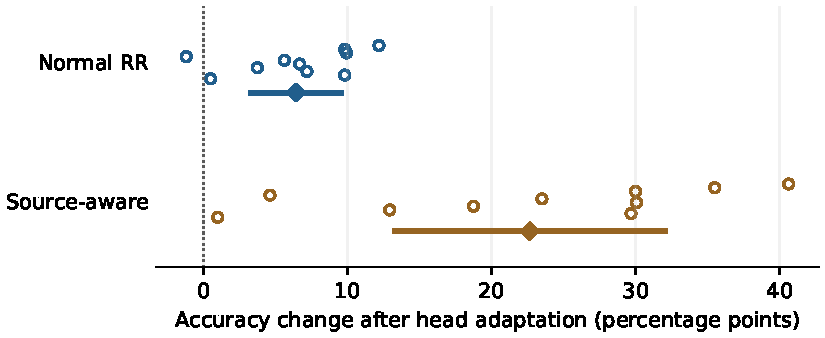
\includegraphics[width=\linewidth]{receiver_adaptation.pdf}
\caption{Change in acting accuracy on new broadcast episodes after fitting follower heads. Circles show each training seed's gain over the unchanged head, diamonds the ten-seed mean, and bars paired 95\% $t$ intervals. Normal RR supplies a current source update on 40\% of steps. Source-aware selection supplies it on all steps and incurs extra diagnostic CPU cost.}\label{fig:adaptation}
\end{figure}
\subsection{When does a traffic saving change the information received?}
On ten slow-trained Full checkpoints, we matched cache decay under Full and RR at both $\lambda=1$ and $\lambda=0.9$ and used 20 paired resets per seed. All 400 paired episodes had identical delivered sender histories, cache tensors, actions, rewards and return. Full offered five 48-byte packets per step and RR offered one. Both delivered one 32-byte payload. Thus the entire 80\% saving can be traced to attempts that Full made after the usable slot had been filled.
\paragraph{When the interpretation changes}
With matched weights, cache rules, initial controller/environment states and exogenous randomness, identical sender-keyed payloads and source timestamps at each step imply identical receiver inputs. The actions, state transitions and rewards then coincide by induction. In the fixed-readiness serial queue, suppose Full and RR can deliver exactly $k$ of $N$ equal-sized packets at every step. With no admission failures and a zero initial cursor, their respective starting positions are $t$ and $kt$ modulo $N$. For $1\leq k<N$, their contiguous sender sets agree when $(k-1)t=0\bmod N$. The guarantee for $k=1$ thus has a specific dependence on ordering. The proof concerns received payloads and timing at the controller. Accounting charges the full offered size of a late packet.

Changing only the access rule at the one-packet boundary also matters. On the same frozen Full weights, DAC cuts offered bytes per step by the same 80\% as RR but changes the sender history in every pair. With matched decay $\lambda=1$ the paired DAC-minus-Full return is $-1.95$ per episode (unadjusted 95\% seed interval $[-3.21,-0.69]$); at $\lambda=0.9$ it is $-1.80$ ($[-2.98,-0.62]$). These are fixed-policy deployment comparisons. Independently training the policies under each rule asks a different question.

We read the same ten frozen Full checkpoints at Medium/2 ms in three ways. First, switching to RR cuts offered bytes per step by 60\%, and episodic return is identical in 259 of 400 pairs. Second, comparing trajectories shows that 222 of those 259 equal-return pairs have different action histories. Third, inspecting the first delivery divergence reveals that Full and RR supply two packets at each common step but first supply different senders at $t=1$ in every pair. Complete count histories match in 349 pairs because episode durations can also differ. An unchanged score therefore misses behavioral change, and action divergence alone leaves its upstream cause unresolved. Matching the checkpoint, reset, cache rule and preparation time localizes the first discrepancy to the information delivered at the second decision. The uniform-subset intervention below estimates its possible consequences on a separate RR/DAC cohort.
\subsection{Sender choice after a common history}
To test selection at the same delivered packet count, we use the ten primary training seeds separately for RR-trained and DAC-trained weights. At prespecified even timesteps along both policies' trajectories, we enumerate every feasible one- or two-sender fresh-message subset, keeping the pre-decision state, policy weights and packet count fixed. Each branch resumes the original access rule thereafter. The best--worst suffix-return range and best-subset regret are hindsight diagnostics, not evidence of performance achievable by an online scheduler. All 2,654 no-op and 2,654 forced-original-subset checks passed. Both compare the full recorded suffix trace: actions, rewards, termination flags, environment states, delivered sender sets, source timestamps and accounted traffic.

The shared-prefix control transmits with RR until every sender is valid, then clones the state and switches to RR or DAC. All prefix traffic and modeled time are included. Episodes ending before full coverage remain in total-return summaries with zero suffix contrast; survivor-only effects are separately reported. This comparison estimates the effect of switching access rules after the same RR history. At the branch point both alternatives inherit the environment state, recurrent state, cache, credit and sender ages as well as the remaining horizon. The experiment cannot attribute the difference between cold-start and prefix comparisons to cache filling alone. Cached-message methods such as TMC~\citep{zhang2020succinct} motivate separating initial acquisition from later refresh.
For each visited state we recorded the range of suffix returns over feasible subsets. At least two feasible subsets gave different suffix returns in 13.94--18.86\% of sampled states across the four policy/link combinations (Fig.~\ref{fig:controlled}). This measures how often a choice could matter. To estimate whether the scheduler used that choice well, we compared its factual subset with the mean over all feasible subsets. Weighting episodes equally, DAC-trained policies gained 0.13 return points on Slow/5 ms (95\% interval $[-0.06,0.32]$) and lost 0.25 on Medium/2 ms ($[-0.64,0.14]$). All four episode-weighted intervals include zero. Two state-weighted intervals exclude zero. The paired effects, sample counts and weighting definitions appear in Supplementary Section~S3.
\begin{figure*}[pos=t]\centering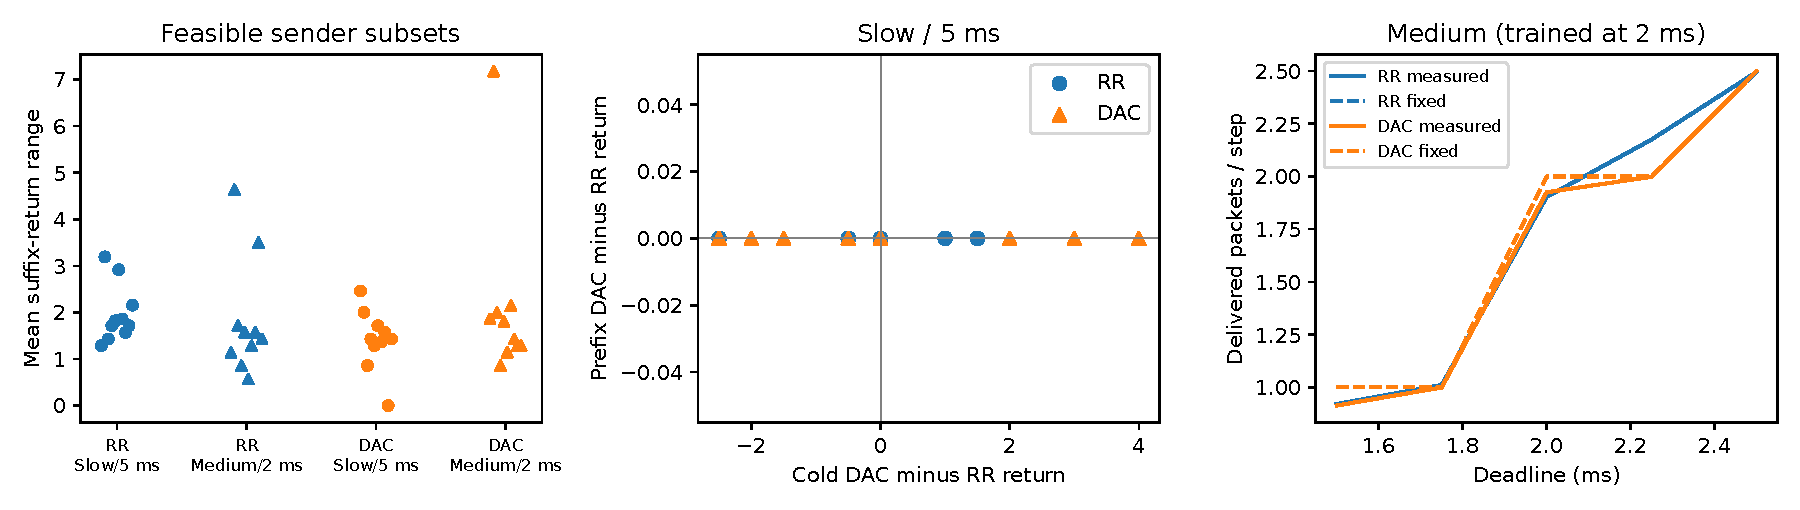
\includegraphics[width=\linewidth]{diagnostics.pdf}
\caption{Primary-checkpoint diagnostics. Left: each point is one seed's mean feasible-subset suffix-return range. Middle: Slow/5 ms only, cold and common-prefix DAC--RR effects on the same frozen policy, with early termination retained. Right: medium link, primary Medium/2 ms-trained RR/DAC checkpoints, mean delivered packets over ten seeds under measured (solid) or fixed (dashed) readiness. Seed-specific curves are retained in the supplementary summary; this panel shows means without uncertainty bands. These are distinct interventions, not pooled training cohorts.}\label{fig:controlled}
\end{figure*}
\paragraph{Switching access rules after the same RR history}
After the common RR prefix, suffix return changes in 0 of 400 Slow/5 ms episodes and 15 of 400 Medium/2 ms episodes. Early termination is retained (Supplementary Section~S3). In the slow condition, 126 pairs nevertheless differ in delivered sets and 94 in actions on common suffix steps. Of 373 survivors, 38 have no unresolved group, 296 have one and 39 have two, with nine steps remaining. An executed global-state action reference verifies unused attainable reward in 335/400 pairs. This reference changes actions and can exploit state unavailable to the deployed policies. Thus identical messages, universal termination and reward saturation do not explain the zero return contrast. The same finite-horizon return can thus hide different later information and actions, even when additional reward remains attainable.

\paragraph{Receiver memory at the same decision point}
A separate intervention crosses the two subsequent access rules with keeping the cache or clearing its payloads and validity timestamps at the same RR-prefix endpoint. We retain the environment state, recurrent state, credit, sender ages, cursor and remaining horizon. In Slow/5 ms we replayed ten RR checkpoints on 20 resets each, keeping the 17 early terminations in the episode averages. All 400 retained-cache suffix checks reproduced the original RR and DAC traces. Clearing memory changed subsequent action histories in 154/200 RR and 155/200 DAC pairs. Every observed suffix return was zero in all four branches. The zero interaction between the reset and the selector therefore reflects a flat return endpoint for these policies. Actions were sensitive to cached information. The return data provide no evidence that initial cache filling mediated the cold-start contrast.
\subsection{Selector computation changes the available channel}
DACOM treats the benefit of waiting for messages as a control decision~\citep{yuan2023dacom}. Here, sender-selection computation consumes time before waiting begins, changing the service opportunity itself. At Medium/2.25 ms, three 48-byte packets require readiness within 310 microseconds, after a 450-microsecond reserve, 50-microsecond propagation and 1.44 ms serialization. RR/DAC mean gate times are 128.7/208.4 microseconds; mean deliveries are 2.175/1.999 packets under measured readiness and 2.000/2.000 under fixed 500-microsecond readiness. Readiness tails and bookkeeping, not mean gate cost alone, determine service opportunities. Thus a nominally identical link does not present both implementations with identical reception opportunities.

\paragraph{Independent-process timing check}
Three independent sequential processes on the same pinned CPU repeat all ten primary seeds at 2.0, 2.25 and 2.5 ms, using three evaluation resets per cell rather than the original ten. At 2.25 ms, RR delivers 2.213, 2.005 and 2.003 packets/step, while DAC delivers 2.000 in all three processes. These repeats put the size of the original packet-count difference in perspective. On identical frozen-policy/input snapshots, DAC's additional gate cost averages 98.5, 99.4 and 100.7 microseconds across these processes, respectively. The extra computation persists, while its conversion into packet loss depends on timing tails and available credit.

\paragraph{How much preparation time is available?}
For a third packet on the Medium link, the preparation budget in microseconds is $D_{\max}-1{,}940$ with $D_{\max}$ expressed in microseconds. At deadlines of 2.00, 2.25 and 2.50 ms this leaves 60, 310 and 560 microseconds. In the original sweep, the percentages of decisions delivering a third packet under RR/DAC were 0/0, 17.5/0 and 49.3/49.8, respectively (average within episode, then within and across seeds). Credit also limits a third transmission. At 2.25 ms, RR's third-packet advantage varied across independent processes. Across identical-input snapshots, DAC added 98--100 microseconds to gate computation under episode-first weighting, with zero paired differences in delivered count on those snapshots. The extra cost changes delivery when it crosses a packet boundary on a step with enough credit. These measurements identify the sensitive region on this host.
\section{Discussion}
\label{sec:discussion}
Table~\ref{tab:evaluation_protocol} sets out the four questions to ask when a lower communication budget appears to preserve return. Which comparison is feasible depends on the task. In MNIST-sum there is a single speaker and no temporal history. In Hallway several senders compete for the same reception slots.
\begin{table*}[pos=t]
\centering\small
\caption{Four-stage evaluation protocol. These are diagnostic controls supported by the present case studies, not a universally validated benchmark standard. Record checkpoints, resets, channel settings and the independent training seeds at every stage. Failed learning checks are reported separately from communication comparisons.}
\label{tab:evaluation_protocol}
\begin{tabularx}{\textwidth}{@{}p{0.14\textwidth}XXX@{}}
\toprule
Stage & Controlled comparison & Required observations & Supported interpretation / decision\\
\midrule
1. Validate the reference & Check learning on held-out data. Where feasible, train ideal-link and no-channel references with matched supervision. For a frozen listener, shuffle or erase the message on the same inputs. & Held-out return or accuracy by seed; learning curves; environment steps; task-solvability reference where available. & Distinguish the effect of giving a training procedure channel access from the effect of a message on an already trained policy. Interpret intervention results only for a qualified reference.\\[3pt]
2. Account for delivery & At fixed weights, resets and cache rule, compare unrestricted attempts with capacity-matched RR. Repeat with measured and fixed readiness. & Offered wire bytes, delivered payload, sender identities and timestamps, waste, CPU time, action deadlines and return. & Identical delivery and control histories with fewer attempts identify traffic savings. Equal nominal caps alone do not establish equal delivery opportunities.\\[3pt]
3. Isolate sender choice & When several senders compete, clone policy, environment and scheduler state and replace the fresh subset at the same received count. Include factual/uniform subsets and a common-initialization control. & No-op and forced-original identity checks; action and suffix-return changes; first delivery and coverage; seed-paired intervals under state and episode weighting. & A paired contrast estimates the total effect of one sender choice under the subsequent original scheduler. Report the effect of switching rules after the shared history and its remaining horizon.\\[3pt]
4. Check downstream use & Compare a held-out probe of the actual receiver input with the acting head; test targeted delivery when task-relevant sources are known. & Decode accuracy, acting accuracy, paired return, actual traffic and diagnostic overhead; task and hardware scope. & A decoder locates accessible information. Roll out the modified acting head on disjoint episodes to test a proposed remedy. Replicate on a learned standard benchmark before extending the result to that benchmark.\\
\bottomrule
\end{tabularx}
\end{table*}
\paragraph{What the controls change}
In MNIST-sum, shuffling messages establishes that the listener uses them. At an equal offered budget, tracking receipt then explains why the listener can tolerate suppressing known late packets and loses accuracy under random thinning. In broadcast, the current source update already reaches the normal receiver often enough to support better decisions. The intervention increased mean episode reward on the original access schedule. Its higher measured action-deadline miss rate remains a cost of the evaluated implementation. In Hallway some same-count sender substitutions change return, but the priority rule has no consistent episode-weighted advantage over a uniform feasible choice. An expensive selector therefore needs evidence of an incremental control benefit in addition to a nominal traffic saving.

\paragraph{Scope and transfer}
The MNIST-sum admission rule knows modeled readiness. Its measured gain does not price online timing prediction. The broadcast receiver adjustment requires training labels, and its accuracy improvement was measured at fixed packet readiness. Hallway's shared-prefix and subset controls require a clonable environment and policy state. Exact enumeration takes $\binom{N}{k}$ suffix rollouts per state. The serial transport model excludes losses, retries, backlog and compute/transport overlap. Centralized score-collection traffic is uncharged, and the timing repeats cover one CPU host.

The XOR reference failed its learning gate in all ten seeds. In SMACv2 an early pilot failed its learning gate and a later three-seed Terran campaign passed at 300,000 steps, but independent-engine replay failed at the second seed after 320 evaluation episodes. Only the separate single-checkpoint technical smoke verified instrumentation (20 episodes and 1,046 steps). These results leave open whether either diagnosis transfers to a learned sequential benchmark. Supplementary Section~S5 reports both the learning and replay outcomes.
\section{Conclusion}
On a learned communication game, two admission rules can spend the same number of bytes and preserve very different amounts of useful information. On a learned broadcast task, the delivery schedule can stay fixed and a change to the receiver can still improve episodic return. The Hallway controls explain why these two observations require different tests. Equal received counts can hide a change of sender, and equal returns can hide a change of action even after a common history. For a particular deployment decision, the evidence must connect the proposed change to what reached the receiver and to what the acting policy did with it.

\section*{Data and code availability}
The accompanying reviewer archive contains the experiment code and configurations, selected policy checkpoints, paired evaluation outputs and verification scripts. It includes instructions and checksums for obtaining the MNIST inputs separately. The supplementary material reports the training and replay settings, seed-level comparisons and unsuccessful validation checks.

\section*{Declaration of generative AI use in manuscript preparation}
OpenAI Codex assisted with drafting, translation, organization and language editing of this manuscript.

\FloatBarrier
\bibliographystyle{cas-model2-names}\bibliography{references}
\end{document}
